\chapter{Турбулентность в системе капиллярных волн на поверхности воды}

Хотя физические параметры жидкого водорода дают некоторые преимущества при экспериментальном изучении слабой волной турбулентности, вода остается удобной для экспериментов с жидкостью. В данной главе представлены экспериментальные результаты исследования волновой турбулентности в системе капиллярных волн на поверхности воды в цилиндрическом и прямоугольном сосудах. Экспериментально было изучено положение высокочастотного края инерционного интервала турбулентного каскада в зависимости от амплитуды накачки монохроматического и широкополосного типа. Так же была оценена характерная частота затухания каскада энергии в диссипативной области для различных амплитуд и спектральных характеристик возбуждающей силы.
\section{Экспериментальная методика} %\label{sect2_1}

Экспериментальная установка, схематично представленная на рис. \ref{img:water_setup}, состоит из виброплатформы 1, установленной на ней экспериментальной ячейки с водой 2 и системы регистрации колебаний 3, 4.
\begin{figure}[ht] 
 \center
 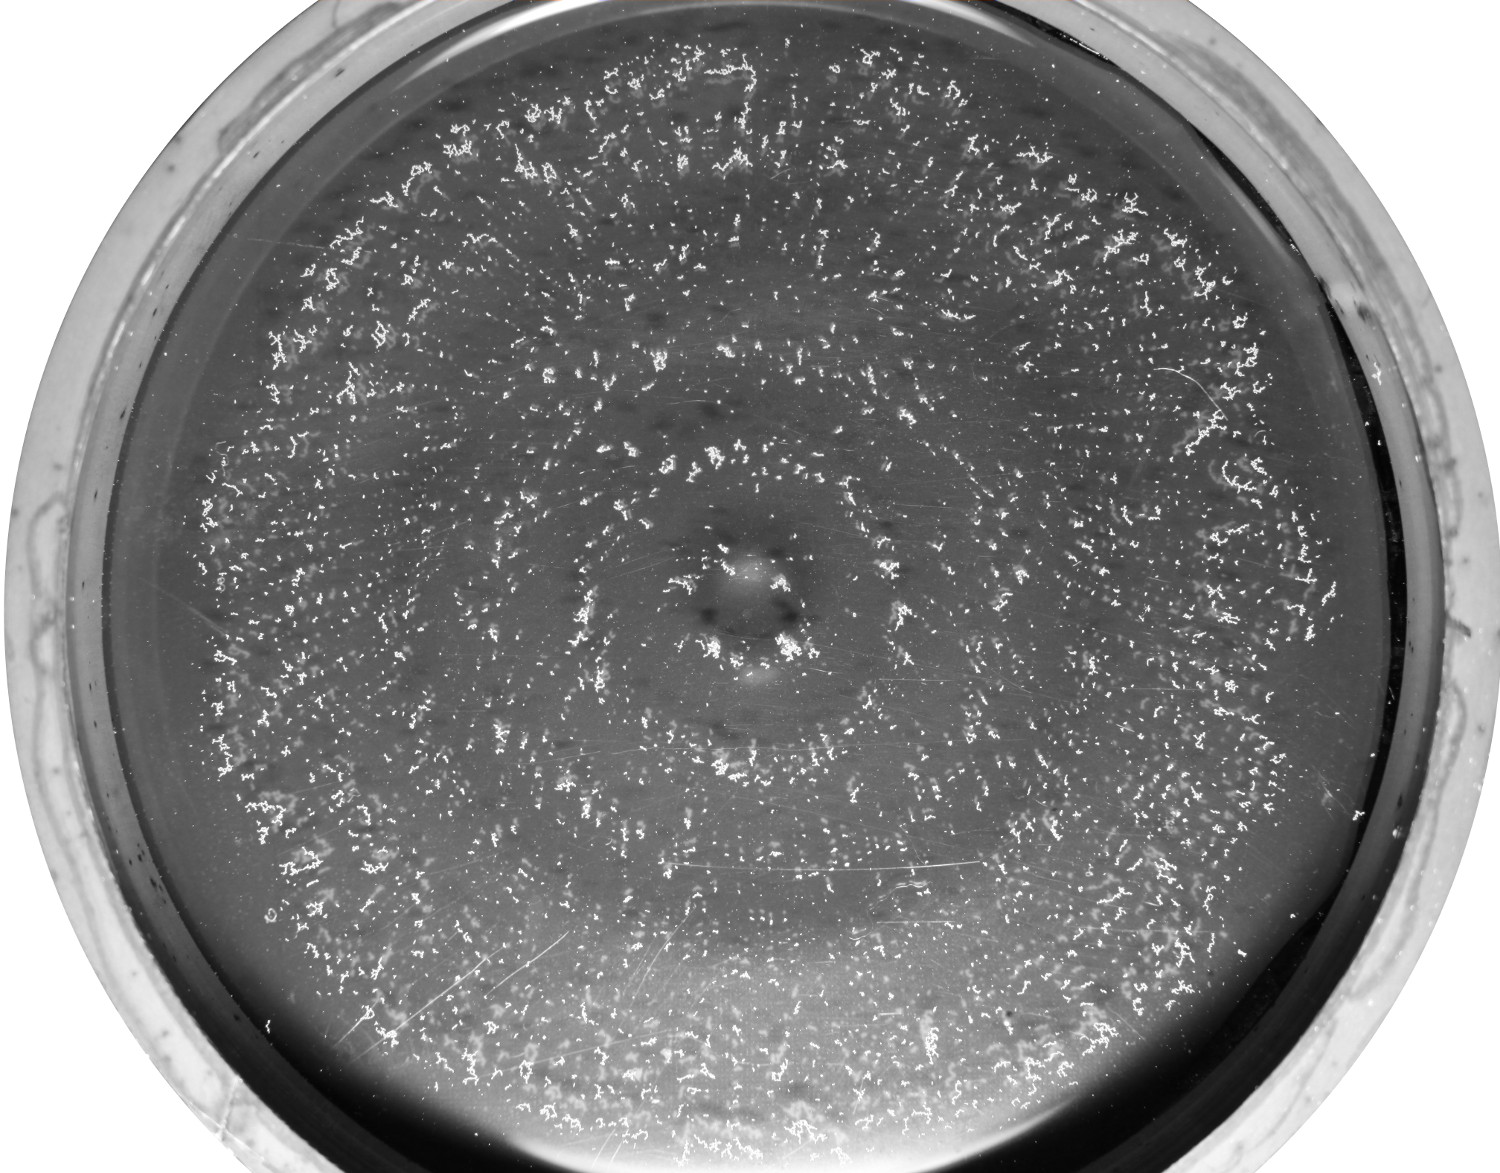
\includegraphics [scale=0.4] {article2/pic_01.jpg}
 \caption{Схема эксперимента: 1 – виброплатформа; 2 – сосуд с водой; 3 – лазер; 4 – фотоприемник.} 
 \label{img:water_setup} 
\end{figure}


Экспериментальные ячейки имели форму стакана с кругом диаметром от 65 до 130 мм или прямоугольником со сторонами 49 $\times$ 50 мм в основании и глубиной 10 мм. Вода наливается выше края стенок стакана так, чтобы образовался выгнутый мениск. При вертикальных осцилляциях ячейки равновесный радиус мениска меняется в зависимости от ускорения ячейки, благодаря чему возбуждаются колебания поверхности воды. 
Колебания ячейки контролировались подачей электрического сигнала с цифрового генератора на вход сабвуфера-виброплатформы.
Использовали следующие виды накачек: монохроматическую на резонансной частоте, узкополосную с шириной полосы около 1 Гц и широкополосную в диапазоне 30–50 Гц. Под амплитудой накачки А в случае монохроматического возбуждения понимается амплитуда электрического сигнала, подаваемого на виброплатформу. В случае узкополосной или широкополосной накачки за амплитуду А принимается среднеквадратичное значение электрического сигнала, подаваемого на виброплатформу. Отметим, что высота волны основной гармоники на поверхности воды прямо пропорциональна амплитуде А (ускорению ячейки в вертикальном направлении) при монохроматической накачке.

Для регистрации колебаний поверхности воды была использована система, ранее описанная в \cite{Brazhnikov_IET}. Скользящий под небольшим углом лазерный луч падает на поверхность воды и отражается от нее. Мощность отраженного лазерного луча зависит от угла отражения. Поэтому присутствие волн на поверхности приводит к временным вариациям мощности отраженного луча $P(t)$. Отраженный луч фокусируется на фотодетектор, электрический сигнал с которого оцифровывается и записывается в память компьютера.

Регистрация волн на поверхности воды происходит в режиме "широкого луча", описанному в разделе \ref{p1_methodDetect}, т.е. характерная длина волн на поверхности воды много меньше размера пятна лазерного луча. Как было сказано выше в этом режиме мощность, регистрируемая фотодетектором, является интегральной характеристикой формы поверхности и при равномерном распределении световой мощности по лазерному пятну на поверхности жидкости парная корреляционная функция $I_\omega$ прямо пропорциональна квадрату компоненты Фурье мощности $P_\omega^2$ отраженного лазерного луча:
\begin{equation}
% \label{eq:disper}
I_\omega = P_\omega^2.
\end{equation}

\begin{figure}[ht] 
 \center
 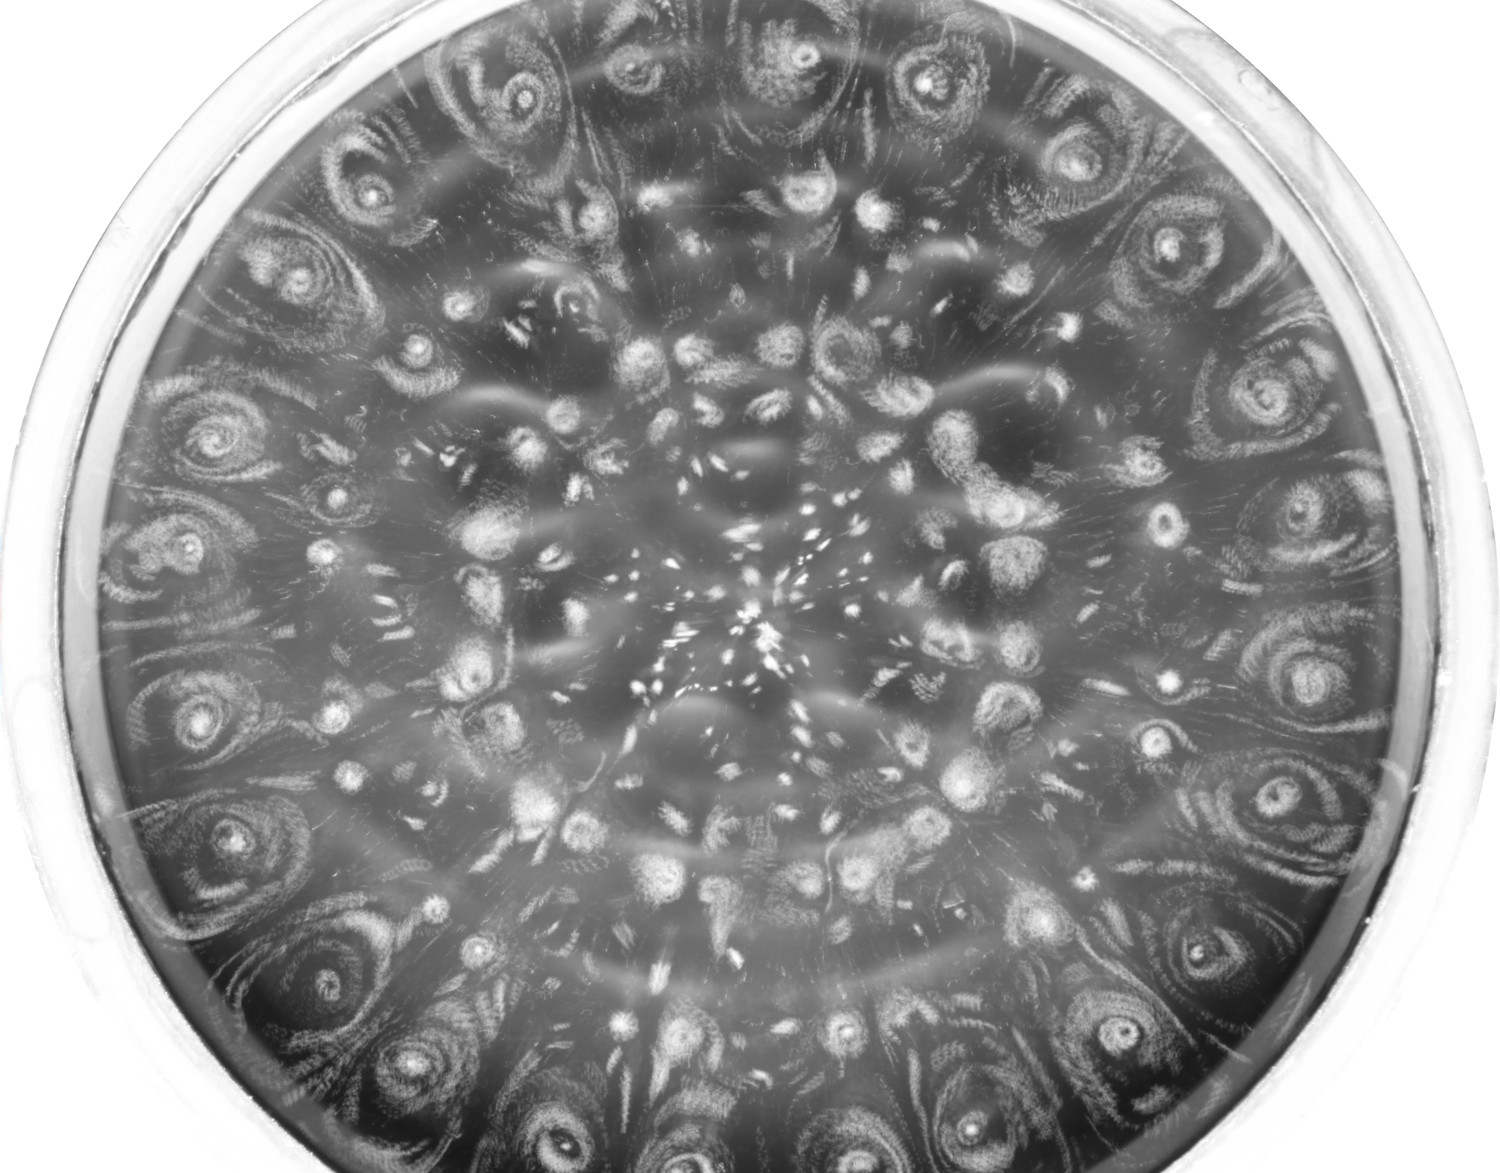
\includegraphics [scale=0.35] {article2/pic_02.jpg}
 \caption{Распределение по частотам и амплитудам волн на поверхности воды в цилиндрической ячейке диаметром 65 мм. Справа приведена шкала амплитуд в произвольных единицах.} 
 \label{img:water_freq_scan} 
\end{figure}


На рис. \ref{img:water_freq_scan} показано экспериментальное распределение амплитуд волн по частоте при возбуждении волн в ячейке диаметром 65 мм, глубиной 10 мм монохроматической силой на фиксированной частоте накачки $f_p$. Частота накачки увеличивается от 46 до 90 Гц с шагом 0.1 Гц. По оси абсцисс отложена частота в герцах, а по оси ординат номер регистрируемой гармоники $N$ с частотой $N f_p$.
Оценка показывает, что в интервале частот от 45 до 90 Гц расстояние между резонансными пиками превосходит ширину пиков, вязкое уширение резонансных пиков $2\nu\omega^{4/3}(\rho/\sigma)^{2/3}$ ($\rho$ – плотность, $\nu$ – кинематическая вязкость, $\sigma$ – коэффициент поверхностного натяжения воды), т.е. спектр поверхностных колебаний в этом диапазоне частот является дискретным.
На рис. \ref{img:water_signal_example} приведен пример записи сигнала, регистрируемого фотодетектором при монохроматическом возбуждении волн на частоте 46 Гц в цилиндрической ячейке. Подчеркнем, что основные вариации мощности отраженного лазерного луча обусловлены колебаниями поверхности воды на частоте накачки.

\begin{figure}[ht] 
 \center
 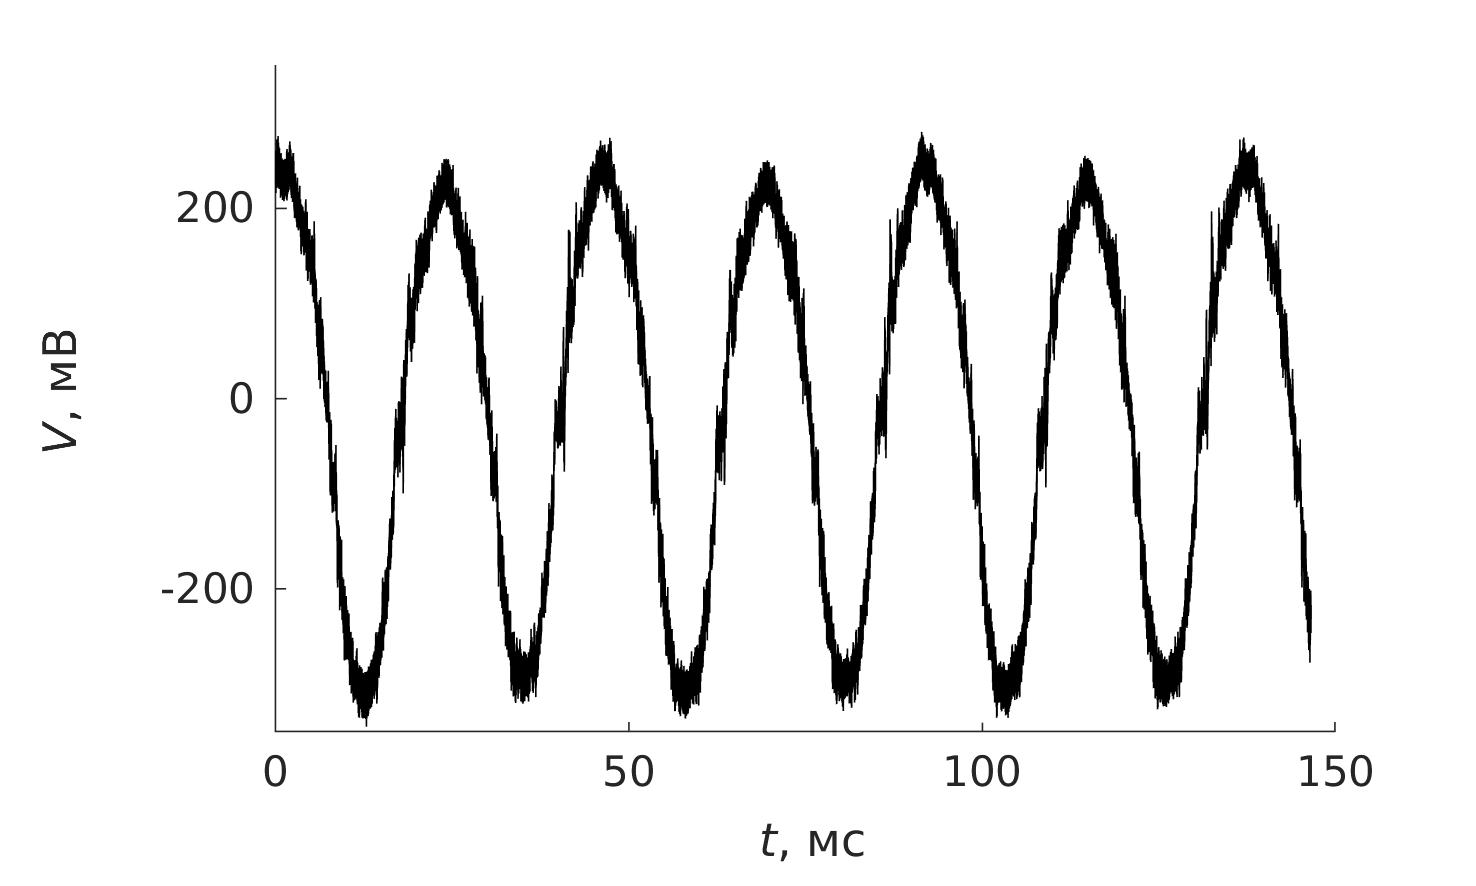
\includegraphics [scale=0.3] {article2/pic_03.jpg}
 \caption{Пример записи сигнала с фотодетектора при возбуждении поверхности воды монохроматической накачкой на частоте 46 Гц в ячейке диаметром 65 мм.} 
 \label{img:water_signal_example} 
\end{figure}




\section{Экспериментальные результаты}% \label{sect2_2}

На рис. \ref{img:water_spectrum} приведен спектр $P^2_\omega$ , полученный Фурье-преобразованием сигнала, фрагмент которого показан на рис. \ref{img:water_signal_example}. Отметим особенности на этом распределении. Самый большой пик, расположенный слева на шкале частот, соответствует частоте возбуждающей монохроматической силы $f_p$ = 46 Гц. Стрелкой на спектре отмечен край инерционного интервала $f_b$. На частотах выше $f_b$ располагается диссипативная область, в которой турбулентный поток энергии быстро затухает. В диапазоне между областью накачки и краем инерционного интервала располагаются пики, соответствующие резонансам, возникшим в результате трехволнового взаимодействия c частотами, кратными $f_b$. Видно, что максимумы пиков в спектре в пределах инерционного интервала хорошо ложатся на прямую линию, которая соответствует степенному закону распределения с показателем степени, близким к -1.8. Значения показателя степени отличается от теоретически предсказанного из-за аппаратной функций экспериментальной методики регистации волн.
\begin{figure}[ht] 
 \center
 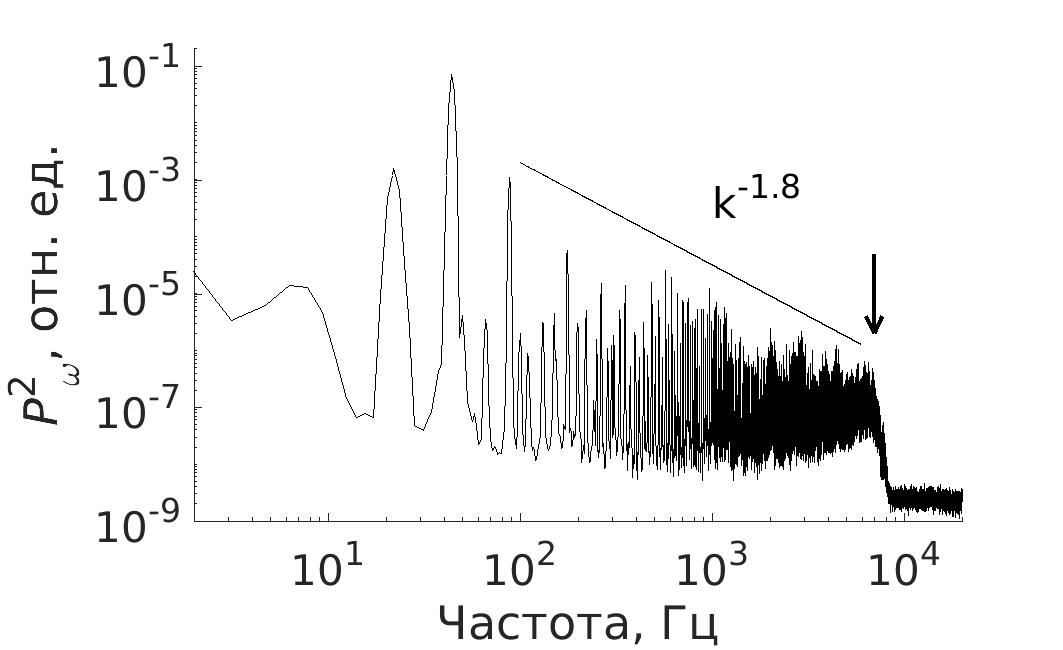
\includegraphics [scale=0.4] {article2/pic_04_new.jpg}
 \caption{Турбулентный каскад на поверхности воды при возбуждении поверхности воды монохроматической накачкой на частоте 46 Гц в ячейке диаметром 65 мм.} 
 \label{img:water_spectrum} 
\end{figure}



С увеличением амплитуды возбуждающей силы положение высокочастотного края инерционного интервала $f_b$ сдвигается в сторону высоких частот. Частота $f_b$ определяется по компенсированным спектрам $P_\omega^2/\omega^\gamma$. Показатель степени $\gamma$ подбирается так, чтобы в инерционным интервале спектр $P_\omega^2/\omega^\gamma$ не зависел от частоты. Значение $f_b$ определяется как частота, при которой отклонение $P_\omega^2/\omega^\gamma$ от плоского спектра составляет 50\%

\section{Высокочастотный край инерционного интервала}% \label{sect2_3}

Анализ зависимостей частоты края инерционного интервала от амплитуды $f_b(A) \sim A^\beta$ показывает, что показатель степени $\beta$ зависит от амплитуды возбуждающей силы. На рис. \ref{img:water_ampl_scan} приведено распределение волн по частотам и амплитудам, полученное при двух последовательных циклах увеличения и уменьшения амплитуды возбуждающей силы на частоте накачки, равной $f_p = 44$ Гц. Край инерционного интервала располагается на границе серого и черного цветов и возрастает по мере повышения амплитуды накачки. На рисунке хорошо видно, что при малых амплитудах накачки частота высокочастотного края инерционного интервала растет по закону немного сильнее линейного, т.е. $\beta > 1$ вплоть до 80-й гармоники частоты накачки. При больших амплитудах накачки показатель степени $\beta$ приближается к единице.

\begin{figure}[ht] 
 \center
 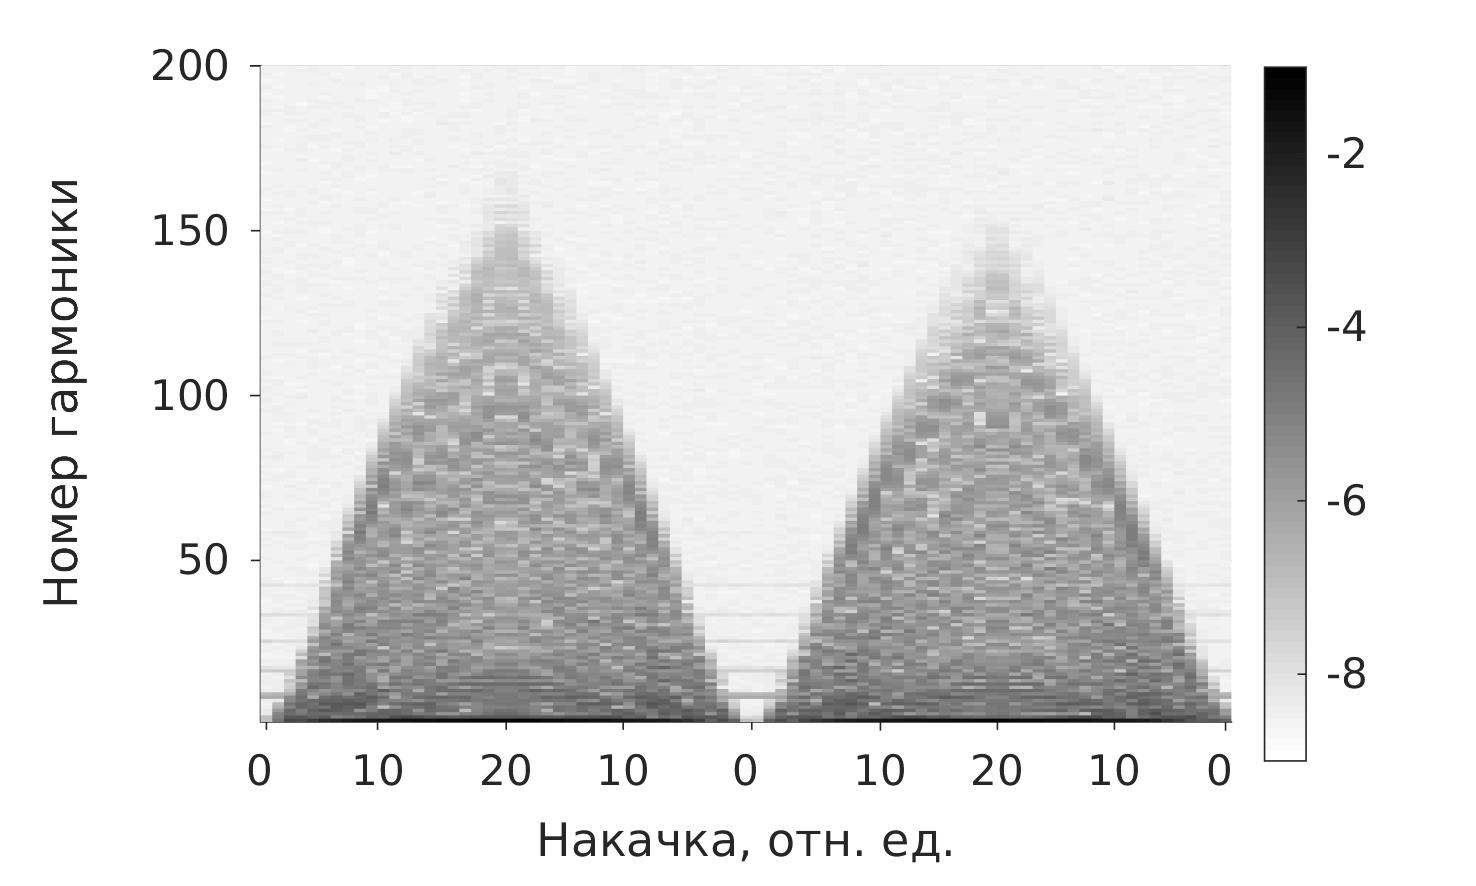
\includegraphics [scale=0.35] {article2/pic_05.jpg}
 \caption{Распределение волн по частоте и амплитуде колебаний при двух последовательных циклах увеличения и уменьшения амплитуды возбуждающей силы на частоте $f_p$ = 44 Гц. Амплитуда возбуждающей силы дана в произвольных единицах. Диаметр ячейки равняется 65 мм.} 
 \label{img:water_ampl_scan} 
\end{figure}

На рис. \ref{img:water_fb_mono} в логарифмическом масштабе приведены зависимости частоты края инерционного интервала $f_b$ от амплитуды монохроматической накачки, полученные в цилиндрической ячейке диаметром 65 мм при накачке на частоте 45.5 Гц, в цилиндрической ячейке диаметром 130 мм при накачке на частоте 44 Гц. Видно, что полученные точки $f_b$ на графиках в логарифмических координатах хорошо ложатся на прямую линию, что соответствует степенной зависимости частоты края инерционного интервала от амплитуды накачки $f_b \sim A^\beta$. Экспериментально полученные значения показателя степени $\beta$ лежат в интервале от $1.23 \pm 0.10$ для всех цилиндрических ячеек. Отметим, что теоретическое значение $\beta$ равно 4/3 для монохроматической накачки \cite{F2}. Таким образом, можно заключить, что экспериментальные значения находятся в согласии с теоретической оценкой.

\begin{figure}[ht]
 \begin{minipage}[ht]{0.49\linewidth}
 \center{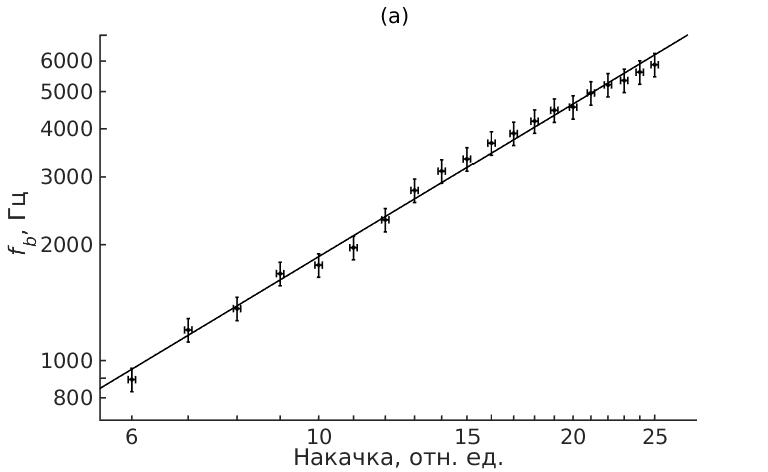
\includegraphics[width=1\linewidth]{article2/pic_06a.jpg} \\ а)}
 \end{minipage}
 \hfill
 \begin{minipage}[ht]{0.49\linewidth}
 \center{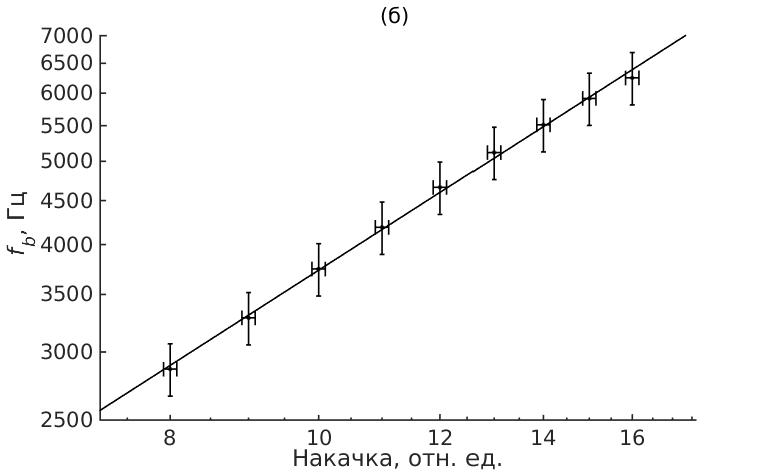
\includegraphics[width=1\linewidth]{article2/pic_06b.jpg} \\ б)}
 \end{minipage}
 \caption{Зависимость высокочастотного края инерционного интервала от амплитуды монохроматической накачки в цилиндрических ячейках диаметром 65 мм, $f_p$ = 45.5 Гц (а) и 130 мм, $f_p$ = 44.0 Гц (б). Прямая линия соответствует степенной зависимости частоты от амплитуды накачки с показателем степени $\beta = 1.32$ для рисунка (а) и $\beta = 1.14$ для рисунка (б)}
 \label{img:water_fb_mono} 
\end{figure}

При переходе от монохроматической к широкополосной накачке также наблюдаются хорошие степенные зависимости $f_b \sim A^\beta$ в широком интервале амплитуд возбуждающей силы, но показатель степени $\beta$ меньше, чем в случае монохроматической накачки.

\begin{figure}[ht]
 \begin{minipage}[ht]{0.49\linewidth}
 \center{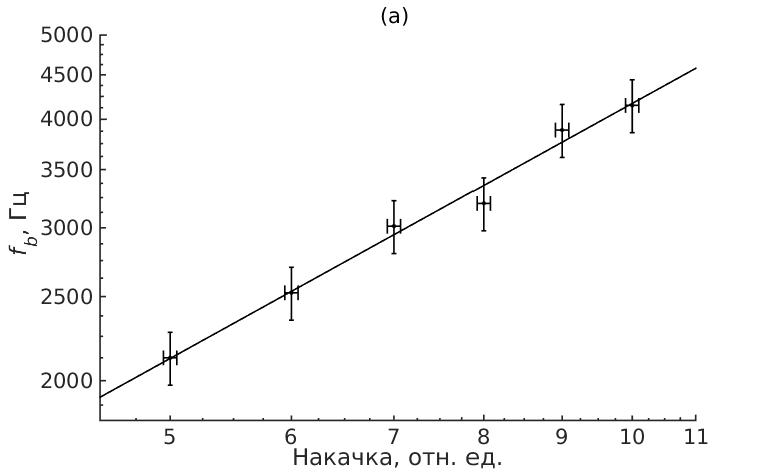
\includegraphics[width=1\linewidth]{article2/pic_07a.jpg} \\ а)}
 \end{minipage}
 \hfill
 \begin{minipage}[ht]{0.49\linewidth}
 \center{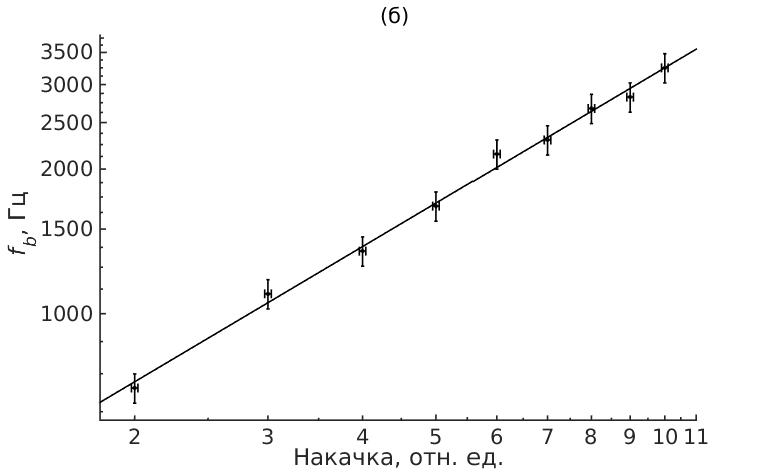
\includegraphics[width=1\linewidth]{article2/pic_07b.jpg} \\ б)}
 \end{minipage}
 \caption{Зависимость высокочастотного края инерционного интервала $f_b$ от амплитуды широкополосной накачки в интервале 30–50 Гц в цилиндрических ячейках диаметром 65 (а) и 130 мм (б). Прямая линия соответствует степенной зависимости частоты от амплитуды накачки с показателем степени $\beta = 0.97$ для рисунка (а) и $\beta = 0.94$ для рисунка (б)}
 \label{img:water_fb_wide} 
\end{figure}

На рис. \ref{img:water_fb_wide} приведены в логарифмическом масштабе зависимости частоты края инерционного интервала от амплитуды широкополосной накачки в диапазоне 30-50 Гц для двух ячеек. Видно, что экспериментальные точки хорошо описываются степенными функциями амплитуды. Показатель степени $\beta$ изменяется от 0.97 в ячейке диаметром 65 мм до 0.94 в ячейке диаметром 130 мм, в среднем $\beta = 0.96 \pm 0.02$.

Также как и в случае монохроматической накачки экспериментальные точки на графиках хорошо ложатся на прямую линию, что соответствует степенной зависимости частоты края инерционного интервала от амплитуды накачки. Отметим, что полученные величины показателя степени $\beta$ составляют в среднем $\beta = 0.96 \pm 0.02$ и значительно отличаются от теоретического значения, равного 12/5 \cite{Ryzhenkova1990}.

Чтобы убедиться, что полученные степенные зависимости $f_b(A)$ не являются особенностью волн в цилиндрической 
ячейке, эксперименты были повторены на почти квадратной ячейке со сторонами $49 \times 50$ мм. На рис. \ref{img:water_fb_rect} приведены зависимости частоты высокочастотного края инерционного интервала $f_b$ от амплитуды монохроматической и широкополосной возбуждающей силы. Видно, что в этих случаях зависимость $f_b(A)$ можно также описать степенной функцией с показателем степени, равным $0.94 \pm 0.02$. В главе 3 будет показано, что при таком возбуждении капиллярные волны формируют вихревые течения, однако оказалось, что присутствие вихрей на поверхности не оказывает существенного влияния на волновую турбулентность.
\begin{figure}[ht]
 \begin{minipage}[ht]{0.49\linewidth}
 \center{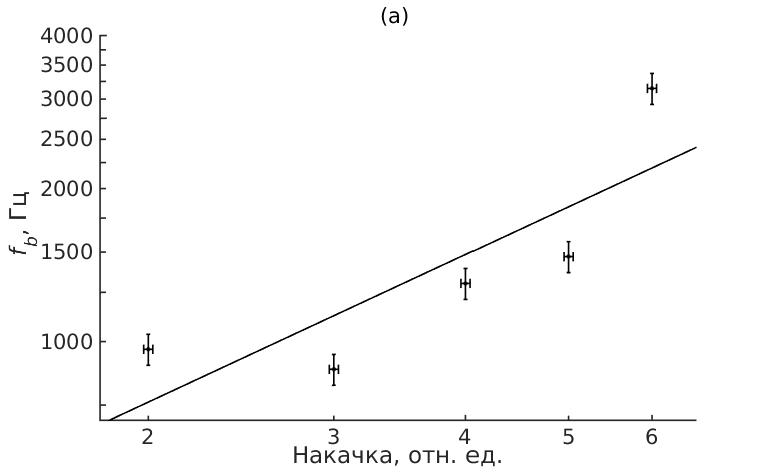
\includegraphics[width=1\linewidth]{article2/pic_08a.jpg} \\ а)}
 \end{minipage}
 \hfill
 \begin{minipage}[ht]{0.49\linewidth}
 \center{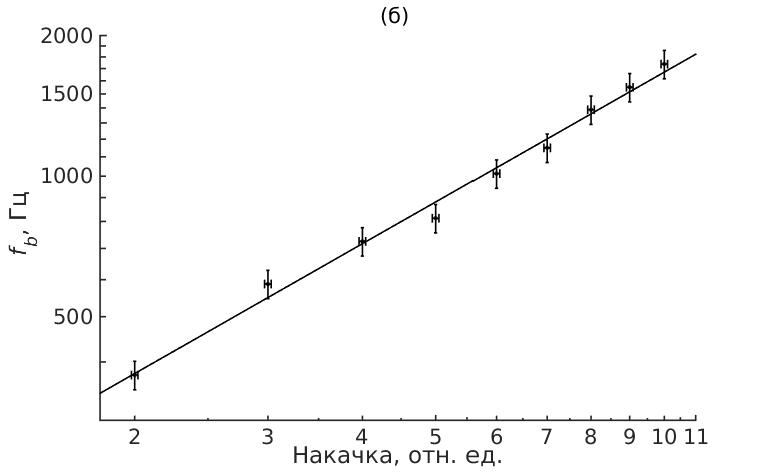
\includegraphics[width=1\linewidth]{article2/pic_08b.jpg} \\ б)}
 \end{minipage}
 \caption{Зависимость частоты высокочастотного края инерционного интервала $f_b$ от амплитуды монохроматической на частоте 42 Гц (а) и широкополосной (б) накачки в диапазоне30-50 Гц в ячейке размерами 49 x 50 мм.  Прямая линия соответствует степенной зависимости частоты от амплитуды накачки с показателем степени $\beta = 0.96$ для рисунка (а) и $\beta = 0.92$ для рисунка (б)}
 \label{img:water_fb_rect} 
\end{figure}

Отметим, что при узкополосной накачке (ширина полосы ~1 Гц) в полученных спектрах $P^2_\omega$ край инерционного интервала слабо выражен, вследствие чего зависимость края инерционного интервала от амплитуды накачки установить не удается.

\section{Характерная частота затухания}% \label{sect2_3}
Как отмечалось выше, на частотах выше $f_b$ турбулентный каскад затухает в результате вязких потерь. На рис. \ref{img:water_fd_mono} в двойных логарифмических координатах приведены зависимости характерной частоты $f_d$ от амплитуды монохроматической накачки для двух ячеек. Отметим, что в ячейке диаметром 65 мм (рис. \ref{img:water_fd_mono}а) частота $f_d$ возрастает по степенному закону при повышении амплитуды возбуждающей силы до относительного значения А = 12. В ячейке большего диаметра так же наблюдается монотонное повышение характерной частоты с ростом уровня накачки. Приближение экспериментальных данных степенной зависимостью $f_d \sim A^\alpha$ дает следующее значения показателя степени $\alpha = 1.18$ для ячейки диаметром 65 мм на растущем участке и $\alpha = 1.38$ для ячейки диаметром 130 мм, в среднем $\alpha = 1.28 \pm 0.10$.

\begin{figure}[ht]
 \begin{minipage}[ht]{0.49\linewidth}
 \center{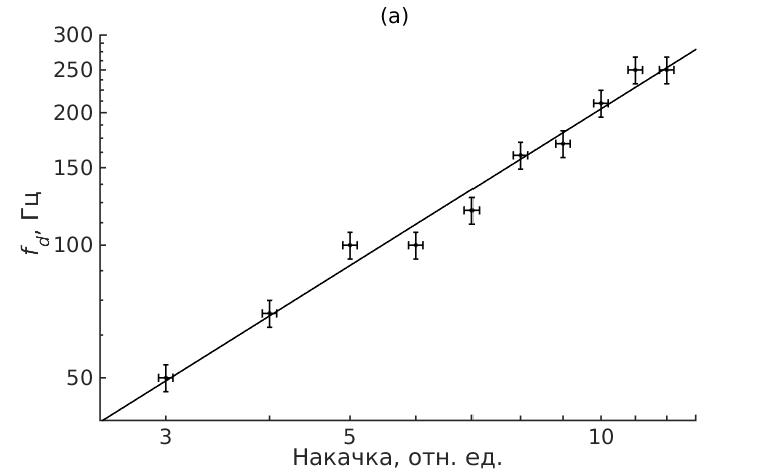
\includegraphics[width=1\linewidth]{article2/pic_09a.jpg} \\ а)}
 \end{minipage}
 \hfill
 \begin{minipage}[ht]{0.49\linewidth}
 \center{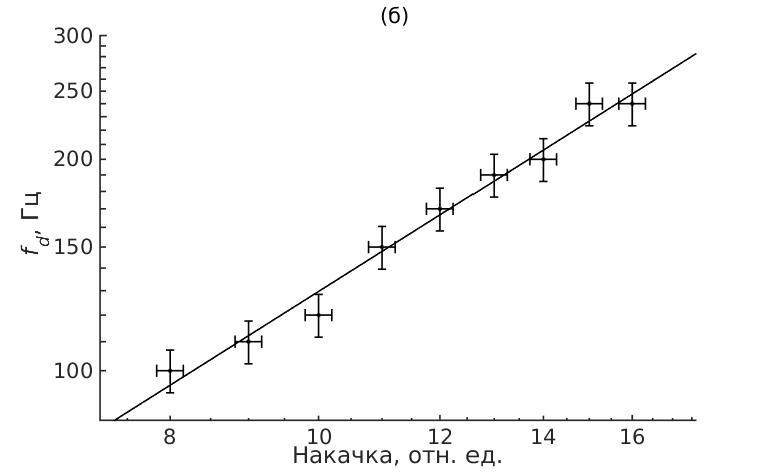
\includegraphics[width=1\linewidth]{article2/pic_09b.jpg} \\ б)}
 \end{minipage}
 \caption{Зависимость характерной частоты $f_d$ от амплитуды возбуждающей силы при монохроматической накачке на частоте 45.5 Гц в ячейке диаметром 65 мм (а) и на частоте 44.0 Гц в ячейке диаметром 130 мм (б).  Прямая линия соответствует степенной зависимости частоты от амплитуды накачки с показателем степени $\alpha = 1.18$ для рисунка (а) и $\alpha = 1.38$ для рисунка (б)}
 \label{img:water_fd_mono} 
\end{figure}

На рис. \ref{img:water_spectra_linear} показано распределение $P^2_\omega$ в полулогарифмических координатах при широкополосной накачке в диапазоне 30–50 Гц, полученное в ячейке диаметром 65 мм. Амплитуды накачки в относительных единицах составляют 3:7:10. Стрелками на каждом спектре показано положение края инерционного интервала $f_b$, которое составляет 650, 2500 и 4300 Гц соответственно. На частотах выше $f_b$ в диссипативной области наблюдается экспоненциальное затухание. Для наглядности на рисунке проведены прямые линии, подчеркивающие экспоненциальные зависимости $P^2_\omega$. Характерные частоты, рассчитанные по зависимостям (2) для распределений, показанных на рис. \ref{img:water_fb_rect}, составляют 430, 1050, 1550 Гц соответственно.

\begin{figure}[ht] 
 \center
 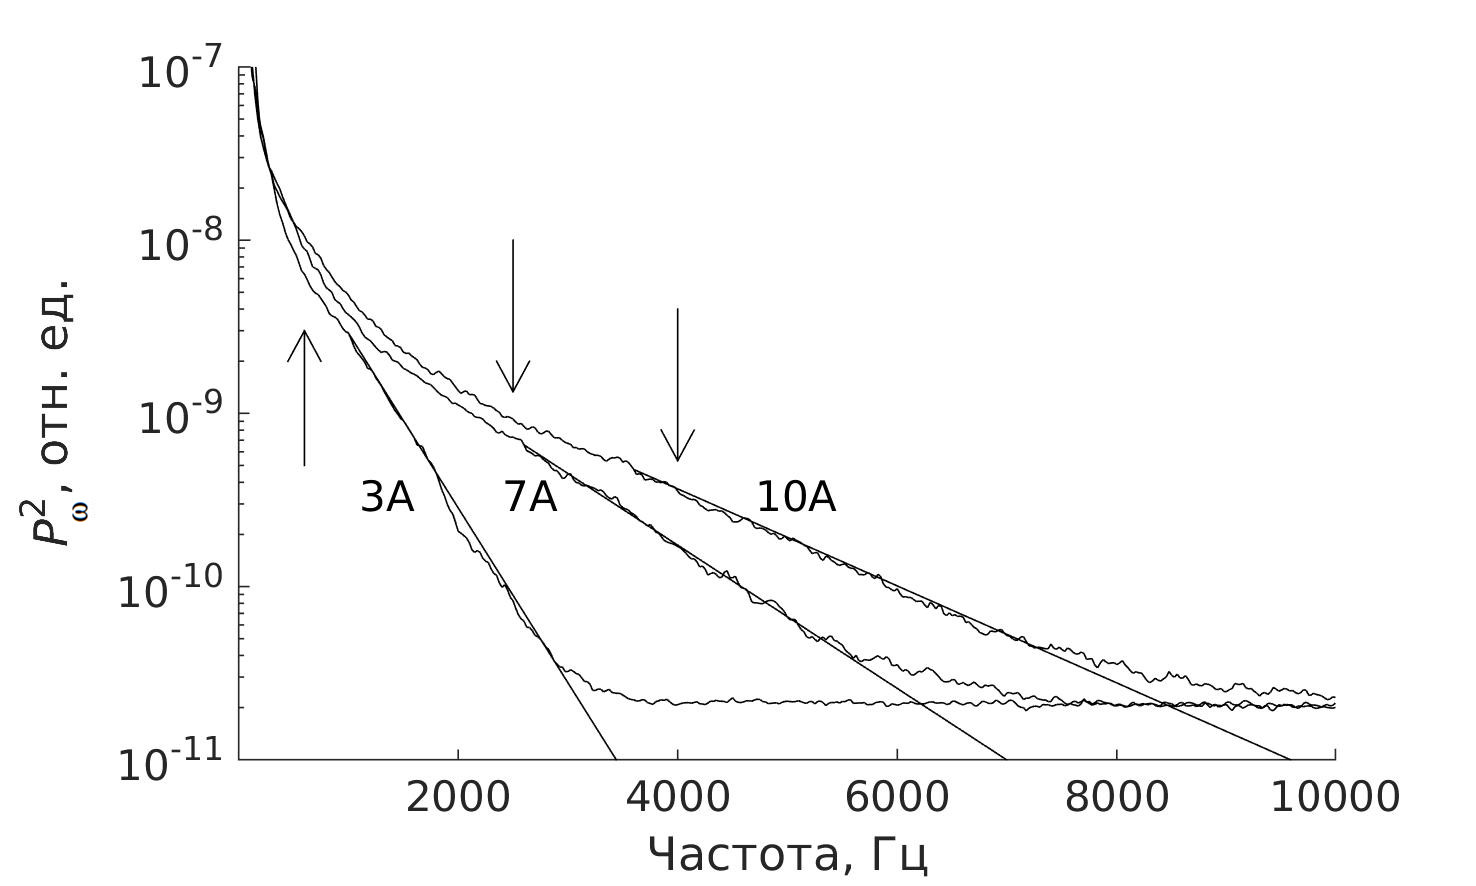
\includegraphics [scale=0.3] {article2/pic_10.jpg}
 \caption{Турбулентные распределения на поверхности воды в ячейке диаметром 65 мм при накачке в диапазоне 30–50 Гц. Амплитуды накачки в относительных единицах приведены у кривых.} 
 \label{img:water_spectra_linear} 
\end{figure}


В случае широкополосной накачки зависимость частоты $f_d$ от амплитуды накачки является монотонной. На рис. \ref{img:water_fd_wide} приведены в логарифмическом масштабе зависимости $f_d$ от амплитуды широкополосной накачки в двух ячейках. Видно, что точки на графике хорошо ложатся на прямую линию, соответствующую степенной зависимости от амплитуды с показателем степени, близким к значениям, полученным по зависимостям частоты края инерционного интервала от амплитуды накачки. Оцененные значения $\alpha$ близки к 1.1.

\begin{figure}[ht]
 \begin{minipage}[ht]{0.49\linewidth}
 {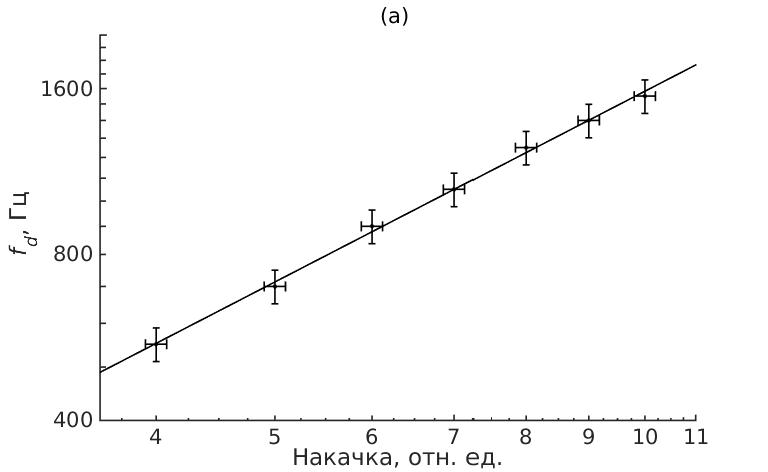
\includegraphics[width=1\linewidth]{article2/pic_11a.jpg} \\ а)}
 \end{minipage}
 \hfill
 \begin{minipage}[ht]{0.49\linewidth}
 {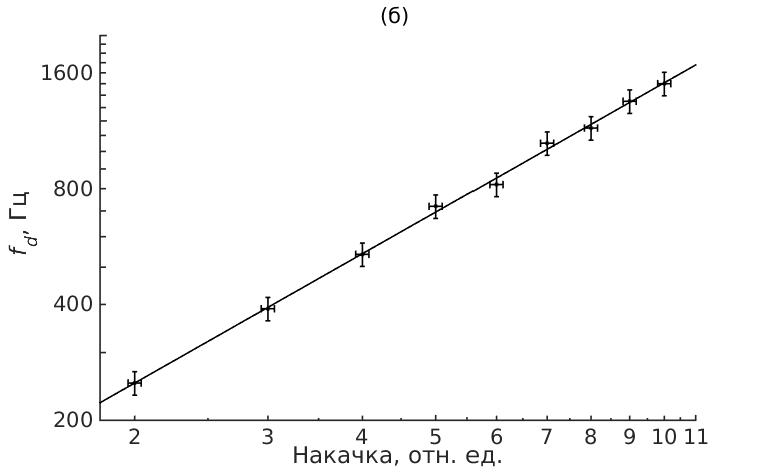
\includegraphics[width=1\linewidth]{article2/pic_11b.jpg} \\ б)}
 \end{minipage}
 \caption{Зависимость характерной частоты $f_d$ от амплитуды возбуждающей силы при широкополосной накачке на частотах от 30 до 50 Гц в ячейке диаметром: а – 65; б – 130 мм.  Прямая линия соответствует степенной зависимости частоты от амплитуды накачки с показателем степени $\alpha = 1.15$ для рисунка (а) и $\alpha = 1.12$ для рисунка (б)}
 \label{img:water_fd_wide} 
\end{figure}


\section{Обсуждение}% \label{sect2_3}

Экспериментальные данные свидетельствуют, что амплитудные зависимости частоты высокочастотного края инерционного интервала $f_b$ можно хорошо описать степенными функциями амплитуды $A^\beta$. Показатель степени при монохроматической накачке составляет в среднем $\beta = 1.23 \pm 0.09$, что близко к теоретической оценке $\beta = 4/3$. Амплитудная зависимость характерной частоты экспоненциального затухания турбулентного каскада описывается степенной функцией с показателем, равным $\alpha = 1.28 \pm 0.10$ Поэтому можно утверждать, что в случае монохроматической накачки частота $f_b$ прямо пропорционально $f_d$, $f_b = m f_d$. Значение коэффициента пропорциональности $m$ составляет 4–5, т.е. характерная частота $f_d$ в несколько раз меньше частоты края инерционного интервала.

При широкополосной накачке показатели степени составляют в среднем $\beta = 0.96 \pm 0.02$ и $\alpha = 1.13 \pm 0.02$. Поэтому можно полагать, что $f_b = n f_d$, а значение n составляет 3–4. Это означает, что гармоники из диссипативной области как при монохроматической накачке, так и при широкополосном возбуждении взаимодействуют, в основном, с модами, расположенными в пределах инерционного интервала \cite{F1}, но ниже частоты его края. Как близко эти моды расположены к краю инерционного интервала, установить сложно, но они значительно выше частоты накачки $f_p$.
Отметим, что в экспериментах со сверхтекучим гелием при монохроматической накачке характерная частота $f_d$ была близка к частоте накачки $f_p$ \cite{F2} и меньше частоты края инерционного интервала в десятки раз. В то же время при широкополосной накачке в экспериментах с жидким водородом характерная частота $f_d$ была только в несколько раз ниже частоты высокочастотного края инерционного интервала $f_b$ и значительно превосходила частоту накачки $f_p$ \cite{F1}.

Таким образом, можно полагать, что отношение частот $f_b$, $f_p$, $f_d$ в экспериментах на поверхности воды, как при широкополосной, так и монохроматической накачке и в экспериментах с широкополосной накачкой поверхности водорода качественно близки. Во всех этих случаях волны из диссипативной области взаимодействуют в основном с модами из инерционного интервала, вдали от областей накачки и края инерционного интервала.

Обратим внимание, что при высоких уровнях монохроматической накачки частота $f_b$ растет с повышением амплитуды по закону слабее линейного (рис. \ref{img:water_ampl_scan}). Остается непонятным расхождение в величине показателя степени $\beta$, полученного в эксперименте и оцененного из теории при широкополосном возбуждении волн. Отметим, что это разногласие наблюдается в экспериментах как с волнами на поверхности воды при различных методиках возбуждения поверхности \cite{BrazhnikovWater}, так и на поверхности жидкого водорода \cite{Brazhnikov_liq_hydr} и сверхтекучего гелия \cite{F2}. Во всех этих экспериментах угловые амплитуды волн на частоте накачки одного порядка, что связано с особенностью методики регистрации отклонения поверхности жидкости от равновесного положения \cite{Brazhnikov_IET}, а кинематическая вязкость жидкостей изменяется примерно в 100 раз. То есть расхождения в значениях $\beta$ не связаны со свойствами жидкостей, а определяются другими причинами. Для прояснения этого вопроса нужны дополнительные исследования.

\section{Выводы} %\label{sect2_4}


В этой главе экспериментально показано, что при возбуждении турбулентного состояния на поверхности воды монохроматической или широкополосной накачкой частота высокочастотного края инерционного интервала и характерная частота вязкого затухания каскада $P^2_\omega$ в диссипативной области отличаются в несколько раз и качественно одинаково повышаются с ростом амплитуды накачки по степенному закону с показателем степени, близким к теоретически оцененному значению для монохроматического возбуждения. В случае широкополосной накачки наблюдается значительное расхождение между экспериментальными и теоретически оцененными значениями показателя $\beta$.

Так же показано, что значения показателя степени слабо зависит от геометрии экспериментальной ячейки.


%\clearpage
